%%%%%%%%%%%%%%%%%%%%%%%%%%%%%%%%%%%%%%%%%%%%
% Chapitre 1
%%%%%%%%%%%%%%%%%%%%%%%%%%%%%%%%%%%%%%%%%%%%

\chapter{The Hubble-Lema\^itre fragmented model: analytical approach} 
\label{Chap:analytical}

In this chapter we introduce the \HubLem model, derive the equations governing the expansion and perform a perturbation analysis to investigate the growth of idealized overdensities.

\minitoc

\section{How to build a Hubble-Lema\^itre model}

\subsection{Initial state}

The first step to obtain a HL-fragmented model is to build an uniform sphere model. The N stars, depending on the required membership, have to be distributed randomly in space inside a certain radius, producing an uniform density. This can be achieved by sampling separately the distance to the center and the angular position of each star, in a method analog as used in \cite{Aarseth1974} for a Plummer model. The distance to the center should be sampled from the function:

\begin{equation}
f_R(X) = R_0 X^2
\end{equation} 

With $R_0$ the bouding radius and X a random variable following a uniform probability law between 0 and 1. A direct uniform law for the radius would overpopulate the outer regions. The angles $\phi$ and $\theta$, respectively azimuthal and polar angle in the physics convention, should be sampled from:


\begin{align}
f_\phi(X_1) & = 2\pi X_1\\
f_\theta(X_2) &= \arccos{ (X_2) }
\end{align}

With $X_1$ following a uniform probability law between 0 and 1 and $X_2$ between -1 and 1. The cartesian coordinates are then found:

\begin{align}
x &= R \sin{\theta} \cos{\phi}\\
y &= R \sin{\theta} \sin{\phi}\\
z &= R \cos{\theta} \\
\end{align}

The N particles are then homogeneously distributed in space in a sphere of radius $R_0$. The next step is to attribute velocities. Unlike other models like the Plummer model, the velocities are here straightforward. We use the Hubble-Lema\^itre velocity field of neighbouring galaxies: velocities are radial from the Milky Way, larger with increasing distances, taking the form:

\begin{equation}
\label{Eq:1_Hubble}
\bold{v} =  \textrm{H}_0 \bold{r},
\end{equation}

with H$_0$ being an equivalent of the well-known Hubble parameter. An appropriate H$_0$ to obtain a fragmented subvirial model has to be inferior to $\sqrt{2}$ (see next section). The model obtained from this is then evolved through a nbody integrator, which in this case is NBODY6.


\subsection{Fragmentation}
\label{Sec:1_apextime}

The cluster expands, driven by the initial Hubble-Lema\^itre velocity field. During this expansion, poissonian fluctuation in density from the uniform model starts to grow: parts of the cluster with more mass initially attract more stars, forming clumps, clumps merge, spontaneously building substructure. These clumps will be analyzed in another section. If the system is bound, the expansion stops at some point, the apex, at which the initial kinetic energy has been spent and converted to potential energy: the cluster is now larger, substructured and subvirial, about to collapse. The apex time $t_a$ of the end of the expansion and the critical value of H$_0$ can be derived from Newton's second law applied to an expanding spherical shell of matter.

We start from a uniform sphere of radius $R_0$, total mass $M$. We consider spherical shells as mass elements, situated at distance $r$ from the origin. As previously said, they are attributed a radial velocity following (for the shell at $r=R_0$) $\bold v_0 = \Hub_0 \bold R_0 = \Hub_0 R_0 \bold u_r$. We want to follow the radial motion of the last shell of mass m, situated at $R$ from the origin. Newton's second law gives:


%\begin{equation}
\begin{align}\label{eq:newton}
m \frac{dv}{dt} & = - \frac{G M m}{R^2}
\end{align}
%\end{equation}

By multiplying on both sides by $v$ and integrating between a given time and $t=0$, one finds

\begin{equation}
v^2(t) - v^2_0 = 2GM \left( \inv{R} - \inv{R_0} \right).
\end{equation}

We take $\nu = v/v0$,  $x= R/R0$ and define:

\begin{equation}
\label{Eq:1_Estar}
E_\ast = \frac{2GM}{R_0 v_0^2}
\end{equation}
which is a dimensionless measure of the total energy of the system. It comes

\begin{equation}
\nu^2  = 1 + E_\ast \left( \inv{x} - 1 \right) .
\end{equation}

The evolution of the system has 3 outcomes, depending on the value of $E_\ast$:
\begin{itemize}
\item $E_\ast<1$ The velocity is always strictly positive as the system expands ($x->\infty$). The system is unbound.
\item $E_\ast=1$ The velocity approaches zero as the system expands. The expansion "stops at an infinite radius". The system is marginally bound.
\item $E_\ast>1$ The velocity reaches zero for a finite radius, the system is bound and will collapses back on itself once the expansion stops. 
\end{itemize}

Using H\'enon units, $G=1$ and $M=1$, and we choose $R_0$=1. Which gives a critical value $E_*$ to have a bound system: $E_* = \frac{2}{\Hub^2_0} < 1$. This means to have a bound system, which stops expanding at some point, one must have $\Hub_0 < \sqrt{2}$.
We only consider in the following the case in which $E_\ast<1$. We have the expression

\begin{equation}
\nu = \sqrt{1+E_\ast\left(\inv{x} - 1\right)}
\end{equation}
which, when derived over time gives

\begin{equation}
\frac{d \nu}{dt} = - \frac{E_\ast}{2 x^2} \left[ 1 + E_\ast\left(\inv{x} -1\right)\right]^{-\frac{1}{2}} \frac{dx}{dt}.
\end{equation}

Combining this with (\ref{eq:newton}), one obtains

\begin{equation}
\frac{dx}{dt} = \Hub_0 \sqrt{1+ E_\ast\left( \inv{x} -1\right)}
\end{equation}

which can be rewritten, using $\tilde{\Hub}_0 = \Hub_0 \sqrt{E_\ast-1}$ and $x_t=\frac{E_\ast}{E_\ast-1}$,

\begin{equation}
\frac{dx}{dt} = \tilde{\Hub}_0 \sqrt{\frac{x_t}{x}-1},
\end{equation}

$x_a$ being the extent of the maximum expansion as we assumed a bound system. The subscript a is for apex. If we choose the notation $u = \frac{x}{x_a}$:

\begin{equation}
\sqrt{\frac{u}{u-1}} \frac{du}{dt} = \frac{\tilde{\Hub}_0}{x_a}
\end{equation}

We know that $x$ varies from 1 to $x_a$, thus $u$ varies from $1/x_a$ to 1. We can then make the change of variable $u = \sin^2\theta$ and separate the variables to get

\begin{equation}
\sqrt{\frac{\sin^2\theta}{1-\sin^2\theta}} 2 \sin\theta \cos\theta d \theta = \frac{\tilde{\Hub}_0}{x_a} dt
\end{equation}

which becomes after simplifications

\begin{equation}
\label{Eq:1_integrand_theta}
[ 1 - \cos(2\theta)]d\theta = \frac{\tilde{\Hub}_0}{x_a} dt .
\end{equation}


We now integrate the expression from $t=0$ to $t$, the time at which the expansions stops and $x$ reaches $x_a$ (wich implies $u_a = 1$ and $\theta_a = \pi /2)$:

\begin{align}
\int^{\pi/2}_{\theta_0} [ 1 - \cos(2\theta)]d\theta  & = \int^t_0 \frac{\tilde{\Hub}_0}{x_a} dt\\
\frac{\pi}{2} - \theta_0 + \frac{\sin(2\theta_0)}{2} & =  \frac{\tilde{\Hub}_0}{x_a} t\\
\pi - 2 \theta_0 + \frac{2}{\sqrt{x_a}}\sqrt{1-\inv{x_a}} & = 2 \frac{\tilde{\Hub}_0}{x_a} t 
\end{align}

which boils down to the expression of the time at which the expansion stops:

\begin{equation}
t_a = \frac{E_\ast \left(\frac{\pi}{2} - \theta_0\right) + \sqrt{E_\ast-1}}{\Hub_0 (E_\ast-1)^{-\frac{3}{2}}}.
\end{equation}

Recalling the quantities:
\begin{align}
E_\ast = \frac{2GM}{R_0 v_0^2}        &;  & x_a=\frac{E_\ast}{E_\ast-1}  &;  &\theta_0 = \sin^{-1}\left(\inv{\sqrt{x_a}}\right)  
\end{align}

See figure \ref{Fig:apextime} for the value of $t_a$ as a function of \Hub$_0$

\begin{figure}
\center
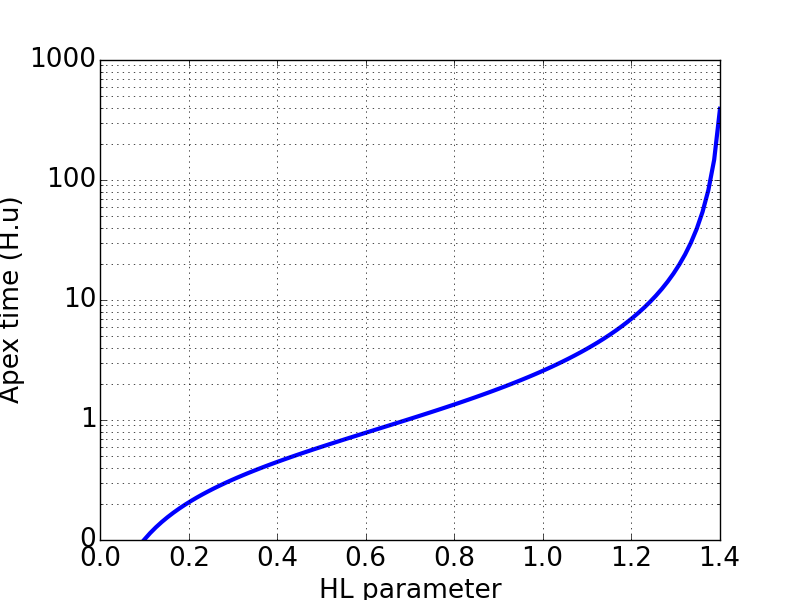
\includegraphics[width=0.7\linewidth]{Figures/1_apextime.png}
\caption{Theoretical values of the apex time, at which the system stops expanding, as a function of initial HL parameter, which tunes the strength of the initial expansion.}
\label{Fig:apextime}
\end{figure} 





\section{The growth of overdensities: analytical study}



\subsection{Working equations}



\begin{table}
\begin{center}
\caption{Summary of main variables.}
\label{Tab:identities}
\begin{tabularx}{\columnwidth}{rl}
\hline
$E$ & Total system energy \\
$E_*$ & Dimensionless total energy \\
$W$ & Total potential energy \\
$E_k$ & Total kinetic energy\\
$\cal M$ & Total system mass\\
$R_o$ & Initial bouding radius\\
$\Hub_0$ & Initial Hubble parameter\\
$v_o$ & Initial velocity at bounding radius\\
$\Hub$ & Variable Hubble parameter\\
$\tau$ & Dimensionless time\\
$x$ & Comoving spatial coordinate\\
$a(t)$ & Rescaling function\\
$\theta$ & Calculation angle\\
$\nu(\tau)$ & Dimensionless velocity $1 + E_*(1/a(\tau)-1)$\\
$\xi$ & Radial displacement from comoving \\
$\delta\rho,\delta M,\delta\rho$ & Perturbed quantities\\
$\mu(\tau)$ & Central point mass\\
$\eta$ & Peculiar velocity $d\xi/dt$\\
\hline
\end{tabularx}
\end{center}
\end{table}

During the expansion and in the mean-field approximation, the mass inside any shell of radius $r(t)$ is conserved as they move outwards. The position of a mass element is known in parametric form from a rescaling of its initial coordinates and we may write 

\begin{align} 
\bold{r}(t) &= a(t)\bold{x}\\
\bold{v}(t) &= \dot{a}\bold{x} = \Hub(t)\bold{r} 
\end{align} 

 where $\bold{x}$ is a co-moving coordinate of position, and $a(t)$ is a dimensionless function of time. The flow is homological and no shell-crossing takes place. It is convenient to introduce a dimensionless time $\tau$ such that 
 
 \begin{equation} 
 \label{Eq:1_taudef}
  t = \frac{\tau}{\Hub_0}.
 \end{equation} 
 
  We then have from equation (\ref{Eq:1_integrand_theta}):
\begin{equation}
\label{Eq:1_Expansion} 
\left. \left[ \frac{ E_\ast}{E_\ast -1} \right]^{\frac{3}{2}} \, \left[ 2\theta - \sin{2\theta} \right]\, \right\vert_{\theta_o}^\theta =  2\sqrt{E_\ast} \tau 
\end{equation}
with 

\begin{equation}  
\label{Eq:1_atheta} 
		a(t)  \equiv  \frac{\sin^2\theta(\tau)} {\sin^2\theta_o}  
\end{equation}


The dimensionless energy parameter $E_\ast$ satisfies  $E_\ast  > 1$ for bound systems. The origin of time $\tau = 0 $ coincides with  the angle $\theta_o$ found from solving 
 $\sin^2\theta_o = (E_\ast - 1) /  E_\ast $. 
%% With $R_o$ and $\Hub_0^{-1}$ dimensional constants for the scales of length and time, repectively, 
The solution (\ref{Eq:1_Expansion})  
provides the time-sequence for the position and velocity of any shell $ 0 < x < R_o$ as parametric functions of $\tau$~: 

\begin{subequations}
\label{Eq:1_HubbleExpr} 
\begin{equation}
 v(t) = \Hub_0 x  \sqrt{ 1 + E_\ast \left( \frac{1}{a(\tau)} - 1 \right) } = \Hub_0 ~ x ~\nu(\tau)
 \end{equation} 
 \begin{equation} 
  \Hub(t) = \Hub_0 ~ \frac{\nu(\tau)}{a(\tau)} 
 \end{equation} 
\begin{equation}
\rho(t) = \frac{3\Mtot}{4\pi R_o^3}\frac{1}{a^3(\tau)}\ . 
\end{equation}			
\end{subequations}

 
\subsection{Linear density perturbation}
\label{Sub:1_FragmentationModes}
An actual Hubble-Lema\^itre model will develop 3-dimensional clumps during the expansion, but to get an analytic view of this process, it is necessary to fall back on one dimension. This will shed light on the growth of clumps and help understand general trends in the system.

We follow radial density perturbations in the expanding uniform sphere described by equations (\ref{Eq:1_Expansion}) and (\ref{Eq:1_atheta}), as the local density increase also gauges the rise in velocity dispersion. A simplified calculation for radial modes of perturbation in the linear approximation will be derived here, with the goal to determine when the clumps become mostly self-gravitating. A more detailed analysis can be found in the classic work by \cite{Friedman1978}, \cite{Peebles1980} and \cite{Aarseth1988} .

We introduce a Lagrangian perturbation in the position of a shell of constant mass by substituting $\mathbf{x} \rightarrow \mathbf{x} + \boldsymbol\xi(\mathbf{x},t)$ and we set $\boldsymbol\xi = \xi \bold{u_r}$ for a radial displacement. Starting from the continuity equation, a linear treatment yields an expression for the perturbed density.

\begin{equation}
\frac{\partial \rho}{\partial t} + \nabla(\rho \bold{v}) = 0 
\end{equation}

which transforms into

\begin{equation}
\delta \rho + \nabla (\rho \bold{v} \delta t) = 0.
\end{equation}

We make use of the equivalence:
\begin{equation}
\label{Eq:1_derivequiv}
\frac{\partial}{\partial r} \equiv \frac{1}{a} \frac{\partial}{\partial x}
\end{equation}

to obtain, considering $ \bold{v} \delta t = \delta \bold{r} = a(\tau) \boldsymbol\xi$ and ignoring second order terms from $\delta \rho$:

\begin{equation} 
\label{Eq:1_DeltaRho} 
\delrho = - \mathbf{\nabla}\cdot (a\rho\mathbf{\xi}) =  - \rho(\tau) \frac{1}{x^2}\frac{\partial}{\partial x} ( x^2\xi ) 
\end{equation}

which leads to a perturbation in  the mass integrated up to  radius $r$ 

\begin{align}
\delta M(<r) &= \delta \left( \rho \frac{4}{3} \pi r^3 \right)\\
    &= - 4\pi a^3(\tau) \rho x^2 \xi . 
\end{align}
Poisson's equation in spherical symmetry gives the perturbed potential 

\begin{equation} 
\label{Eq:1_Poisson} 
\frac{1}{r^2}\frac{\partial}{\partial r} r^2\frac{\partial}{\partial r} \delphi =\frac{1}{a^2}\frac{1}{x^2}\frac{\partial}{\partial x} x^2\frac{\partial}{\partial x} \delphi  = 4\pi G\delrho .
\end{equation}
Substituting for $\delrho$ from (\ref{Eq:1_DeltaRho}) in (\ref{Eq:1_Poisson}), and using (\ref{Eq:1_derivequiv}), we obtain:
\begin{equation}
\frac{\partial}{\partial x} \left( x^2 \frac{\partial \delphi}{\partial x} \right) = - 4\pi a^2 G \rho_0 \frac{\partial}{\partial x} \left( x^2 \xi \right).
\end{equation}
Integrating once, we obtain the general solution
\begin{equation}
\label{Eq:1_Gradpsi} 
a(\tau)\nabla \delphi = \frac{3G\Mtot}{R_o^3} \left( - \xi + R_o^3\frac{\mu(\tau)}{x^2} \right) 
\end{equation}
where $\mu$ stands for a central point mass. A point mass would form by shell crossing at the center of coordinates. In an expanding system, shell crossing at the center is unlikely. For that reason, we make $ \mu = 0$ in the remainder of this paper.

The equations of motion at co-moving radius $x +\xi(x,t)$ can be expanded to first order in $\xi$~; identifying terms of the same order we obtain (with $\partial/\partial x = \nabla_x$)

\begin{equation} 
a(\tau) \frac{d^2}{d t^2} \xi + 2 \dot{a}(\tau) \frac{d}{dt}\xi = - \nabla\delphi - \xi \nabla_x \nabla\phi - \ddot{a}(\tau)\xi \ . 
\end{equation} 
The second and third terms on the right-hand side cancel out exactly~; the first is known from (\ref{Eq:1_Gradpsi}). 
It is standard practice to demote this second-order dynamical equation to a set of first order equations~; for convenience we use the initial system radius $R_o$ as unit of length,  and we introduce starred ($\ast$) dimensionless variables. We then have $x = R_o x_\ast, \xi = R_o\xistar$, and so on.  After simplification using the dimensionless functions of $\tau$  defined in (\ref{Eq:1_taudef}) and recalling that $\dot{a}(\tau) = \textrm{H}(\tau)$, the differential equations read

\begin{subequations}
 \label{Eq:1_system}
    \begin{align}
    	\label{Eq:1_systema}
		\frac{d}{d\tau} \xistar &=  \etastar(\tau)  \\ 
		\label{Eq:1_systemb}
		\frac{d}{d\tau} \etastar &= \frac{3 \Estar}{a(\tau)^2}\,\xistar - 2 		\frac{\textrm{H}(\tau)}{a(\tau)} \etastar   
	\end{align}
\end{subequations}
where we have introduced the peculiar velocity $\eta \equiv d\xi/dt = \Hub_0R_o \eta_\ast$.  


\subsection{Consistent initial conditions} 
\subsubsection{Initial conditions} 
Equations (\ref{Eq:1_system}) can be numerically integrated with an explicit integration scheme once the initial values $R_o, \Hub_0, {\cal M}$ and $\xistar(0)$ are specified and values of $a(\tau)$ are obtained from (\ref{Eq:1_atheta}) and (\ref{Eq:1_Expansion}). All functions of the dimensionless time $\tau$ are set to unity except that $\etastar(0) = 0$. The solution is shown in the next section,  on Fig~\ref{Fig:1_tau_ms}.


The Hubble parameter $\Hub(\tau) \rightarrow 0$ when the system reaches a maximum radius $a(\tau)R_o$ ($\theta[\tau]=\pi/2$ in Eq.~\ref{Eq:1_atheta}). Around that time, equation (\ref{Eq:1_systemb}) transforms so the Lagrangian displacement $\xistar$ grows exponentially, and the clumps become the densest. We investigate the growth of a density perturbation as a Fourier fragmentation mode before that. In the linear regime, such a mode is decoupled from all the others. We pick 

 \begin{figure}
	\center
 	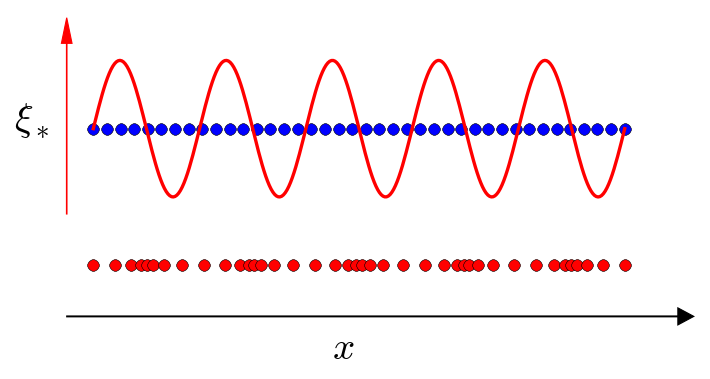
\includegraphics[width=0.7\textwidth]{Figures/1_perturbation.png}
	\caption{Schematic illustration of a sinewave density perturbation (red line) applied to an uniform distribution of matter (blue dots) and the resulting distribution (red dots). The mode displayed here has $m=10$ and its amplitude was exaggerated.} 
	\label{Fig:1_perturbation}
\end{figure}

\begin{equation} 
\label{Eq:1_FourierMode} 
   \xistar(x,0) = \xistaro \sin( kx ) ,
\end{equation}  
where the wavenumber $k$ is such that $k R_o = m \pi$ and $\xistar(R_o,0) = \xistar(R_o,\tau) = 0$ at all times. When deciding which wavenumber to choose, we must bear in mind the finite numerical resolution of the models that we will present later. The next subsection gives quantitative arguments that motivated our choices.  
The aspect of the perturbed system is shown as a rough schematic on Fig~\ref{Fig:1_perturbation}.

\subsubsection{Fourier modes: resolution issues} 
\label{Ssub:1_FourierModes}
An uniform distribution of $N$ discrete mass elements cannot resolve infinitely small wavelengths, the lower limit depends on the mean separation $l_o\simeq R_o / N^{1/3}$ which gives a reference wavelength $\lambda / R_o = \lambda_\ast \ge N^{-1/3}$ for a resolved  Fourier mode. 
Since $kR_o = m\pi$, this also implies that $ m \le 2 N^{1/3}$.  

The initial amplitude $\xistaro$  of the perturbation can be tailored to the actual Poissonian fluctuations in a uniform distribution of discrete elements. The radius bounding a shell of $N$ mass elements distributed randomly will fluctuate freely between $r$, $r + \delta r$ due to stochasticity. The radius $r$ of a uniform sphere being a power-law of mass $M$, we 
find:
\begin{equation}
\frac{\delta r}{r} = \frac{1}{3}\,\frac{\delta M}{M} =  \frac{1}{3}\,\frac{\delta N}{N} = \frac{1}{3} N^{-\frac{1}{2}}
\end{equation}
 for identical mass elements. We then compute the number-averaged value $\langle \delta r/r\rangle$ by summing over  all elements from 1 to $N$ and dividing by $N-1$ to find 
\begin{equation}
\langle \frac{\delta r}{r} \rangle = \langle \xistaro\rangle = \frac{2}{3} \frac{\sqrt{N} - 1 }{N - 1} \ .
\end{equation}  

Thus the mean amplitude (in units of $R_o$) is $\langle\xistaro\rangle\simeq 1/10$ for $N=32$ which drops to $\langle\xistaro\rangle\simeq 6\times 10^{-4}$ when $N = 10^6$. We checked that the mode with the shortest wavelength $\lambda_\ast$ still resolved would have a displacement $\langle\xistaro\rangle$ initially 
smaller than $\lambda_\ast/2$ for any sensible value of $N$. This in turn implies that this mode may grow over time to reach an amplitude $\xistar(x,\tau) \simeq \lambda_\ast/2$, which is the point when orbit-crossing between shells of constant mass must occur. In other words, at this point, the overdensity transitions from linear convergence of particles to  collisional evolution (not covered by Eqs.~\ref{Eq:1_system}). The time when shell-crossing occurs can be seen as the "birth" of a clump, whether this clumps undergoes consequent two-body relaxation effects depends on its characteristics, such as density and membership, and the remaining time before the end of expansion. 

\subsection{Segregation time-scale} 
\label{Sec:Timescales} 
We already noted that $\Hub_0^{-1}$ sets a time-scale for the expansion of the system. That time should be chosen so that it matches the hydrodynamical star formation
phase of $0.5 - 1$ Myr \citep{Maschberger2011,Bate2014}. 
When $\Hub(\tau) = 0$ and the expansion is over, the stars relax to a new equilibrium driven by star-star interactions. Therefore we need to address first the 
internal dynamics in clumps in time units of $\Hub_0^{-1}$, before discussing the later phase of violent relaxation and consider the system as a whole. 
The definitions are the same, only the face values change between the two phases of evolution. 

Let us consider a clump of membership $N_\lambda$ initiated by a Fourier mode of wavelength $\lambda$. With its total density $\rho + \delrho$ given by Eq.~(\ref{Eq:1_DeltaRho}), we may write 

\begin{equation}
 \rho_g = \frac{\rho_o}{a^3(\tau)} \, \left( 1 + \frac{\delrho}{\rho} \right) \equiv  \frac{\rho_o}{a^3(\tau)} \, \rho_\ast.
 \end{equation}
 
Combining this with Eqs.~(\ref{Eq:0_tcr}), (\ref{Eq:0_trel}) and (\ref{Eq:0_ms2}) from the introduction, the mass-segregation timescale in the clump now reads:

\begin{equation}
 \tms = \frac{0.138}{6}\pi \left(\frac{3}{4\pi}\right)^{1/2} \frac{\langle m_\star\rangle}{\max\{m_\star\}} \, \frac{N_\lambda}{\ln 0.4 N_\lambda} \, (G\rho_g)^{-\frac{1}{2}}\, . \end{equation}
  
Making use of the equality 

\begin{equation}
\frac{4\pi}{3} G\rho_o = \Hub_0^2 \Estar ,
\end{equation} 
the last three relations simplify to the expression of the new dimensionless mass-segregation timescale:

\begin{equation}\label{Eqn:Taums} 
\tau_{ms} = \Hub_0 \tms = \frac{0.138}{6} \pi \, \frac{a_\lambda^{3/2}}{(\rho_\ast\Estar)^{1/2}} \, \frac{\langle m_\star\rangle}{\max\{m_\star\}} \, \frac{N_\lambda}{\ln 0.4 N_\lambda} 
\end{equation}
where $a_\lambda$ refers to the expansion factor $a(\tau)$ evaluated at time $\tau$ when $\xistar \simeq \lambda_\ast/2$. Note that our use of Eq.~(\ref{Eq:1_DeltaRho}) to compute $\rho_g$ means that the gravitational radius $r_g$ does not have its usual definition based on the gravitational energy $W$ of the system. Linking 
$\rho_g$ to $R_g$ in this way has the advantage that $R_g$ is not derived from an implied mass profile, which is (by definition) not resolved 
here. 

Clearly the segregation time depends strongly on the mass spectrum of individual clumps, on their membership $N_\lambda$, as well as the density contrast $\rho_\ast(\tau_\lambda)$. We find the density contrast from (\ref{Eq:1_FourierMode}) and (\ref{Eq:1_DeltaRho}),  

\[ \left.\frac{\delrho}{\rho}\right|_{\tau=0} \!\!\!\! = - \frac{1}{x^2}\frac{\partial}{\partial x^2} x^2\xi = - \left( 2 \frac{\sin\, m\pi x_\ast }{m\pi x_\ast} + \cos\,m\pi x_\ast \right) m\pi   \xistaro
\]
which admits an upper-bound of $3 m\pi \xistaro$. In the course of evolution, the initial amplitude of perturbation grows to $\xistar = \lambda_\ast/2$ so that the density contrast peaks at 

\begin{equation} \label{Eqn:Densitypeak} 
  \rho_\ast = 1 + \frac{\delrho}{\rho} = 1 + 3 m\pi \lambda_\ast / 2 = 1 + 3\pi\, ,
\end{equation}
where the last substitution follows from the definition of the integer $m$. The mass $M_\lambda$ in a shell bounded by $r, r+ \lambda$, is known from the unperturbed density profile~; in terms of the total system mass ${\cal M}$, we find 

\begin{equation} \label{Eqn:Clumpmass} 
   \frac{M_\lambda}{{\cal M} } = ( \overline{3 x_\ast^2} + \lambda_\ast^2/4 ) \lambda_\ast = ( 1 + \lambda_\ast^2/4) \lambda_\ast \, , 
\end{equation}
where we have replaced $3x_\ast^2$ by its space-averaged value in  the last step.  Eq. (\ref{Eqn:Clumpmass}) provides an estimate of  bound mass of a clump formed through the growth of a radial perturbation mode. If all the stars have equal masses, or, if the stellar mass function is symmetric with respect to the mean value $\langle m_\ast\rangle$, the ratio of the number $N_\lambda$ of stars in the clump to the total number $N$ is in the same proportion as $\frac{M_\lambda}{\cal M}$. We find an estimate for $N_\lambda$ which reads 

\begin{equation} \label{Eqn:Clumpn} 
   N_\lambda = N \left( 1 + \frac{\lambda_\ast^2}{4} \right) \lambda_* .
\end{equation} 

We argued in \S2.3.2 that a resolved mode should have $\lambda_\ast \ge N^{-1/3}$, which translates as: 

\begin{equation} \label{Eqn:Clumpn} 
   N_\lambda > N^{2/3}\left( 1 + \frac{N^{-2/3}}{4} \right) .
\end{equation}
This number inserted into Eq.(\ref{Eqn:Taums}) leads to a rough picture of the segregation process in clumps. The rate of mass segregation leans  on the choice of initial value for the expansion phase, $\Hub_0$. In the limit when $\Hub_0 = 0$, there is no expansion whatsoever, and the clumps form unsegregated (aside from random associations when attributing positions and velocities to the stars) during global infall. If by contrast, the expansion is vigourous, $a_\lambda \gg 1$, and the segregation timescale remains large. For $N \sim 10^4$, we compute from (\ref{Eqn:Clumpn}) $N_\lambda \gtrsim 464$: a clump with that many stars will mass-segregate rapidly only if its stellar mass function includes very massive stars. We note that one-dimensional (radial) modes would in fact split into several smaller fragments in a three-dimensional calculation.\footnote{ A full-grown radial mode forms a thin shell subject to fragmentation. See \textit{e.g.}  \cite{Ehlerova1997,Wunsch2010}.} We expect  the clumps to form quickly  and contain $N_\lambda \ll 464$ stars, so  that the internal dynamics 
will drive mass segregation {\it before} the system expansion stops. Because this depends in the details on $\Hub_0$ and other important parameters, 
% on the clump stellar mass function, the density contrast reached, and the initial expansion rate, among important parameters, 
we defer the analysis to \S \ref{TODO} and N-body simulations. 
% Still, this simple one-dimensional mode analysis helps to understand the basics of the fragmentation proces



\subsection{Example with N = 15000} 
\label{Sec:HubbleExpansion}
%This section discusses the growth of fragments and their properties at the end of the Hubble expansion phase. Because hydrodynamical calculations of supersonic turbulence show proto-stars forming during a single free-fall time,  
%
%\begin{equation} \label{Eqn:Freefall} 
%   t_{ff} = \left(\frac{3\pi}{32 G\rho_o} \right)^{1/2} \sim 0.5 - 1 {\rm Myr}
%\end{equation}
%(where $\rho_o$ is taken as the global mean density), we should pick a set of parameters such that the clumps form over a physical time to match that of Eq.~(\ref{Eqn:Freefall}). In this work, we choose to evolve the models until $H = 0$ to allow for fully-developed individual clumps. More precisely, we look for a computational setup such that $\Hub(\tau) = 0$ in a minimum of one star-formation timescale $t_{ff}$. We do so although the approach taken here to form clumps would allow to stop the calculation {\it before} $H = 0 $ and {\it subtract} the residual radial velocities using Eqs \ref{Eq:1_HubbleExpr}. As a result, the configuration would be less fragmented than for the case when $H =0$. Thereafter the dynamical evolution would proceed similarly in all the cases, but with different clump mass- and size distributions. The choice of initial Hubble parameter $\Hub_0$ must always yield $E < 0$ in (\ref{Eq:1_Estar}) . Note again that when $\Hub_0$ is set equal to zero, we recover the classic configuration for the cold collapse of uniform bodies.




 \begin{figure}
\center
    \centering
    \begin{subfigure}[b]{0.49\textwidth}
    	\centering
    	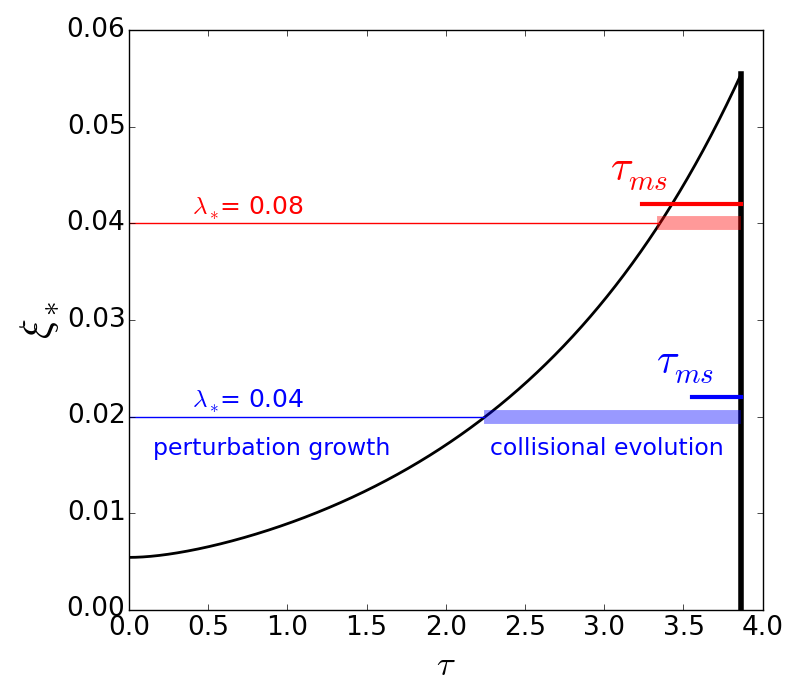
\includegraphics[width=\textwidth]{Figures/1_tau_ms.png}
        \caption{Regimes of overdensity evolution}
        \label{Fig:1_tau_ms}
    \end{subfigure}
    \begin{subfigure}[b]{0.49\textwidth}
    	\centering
    	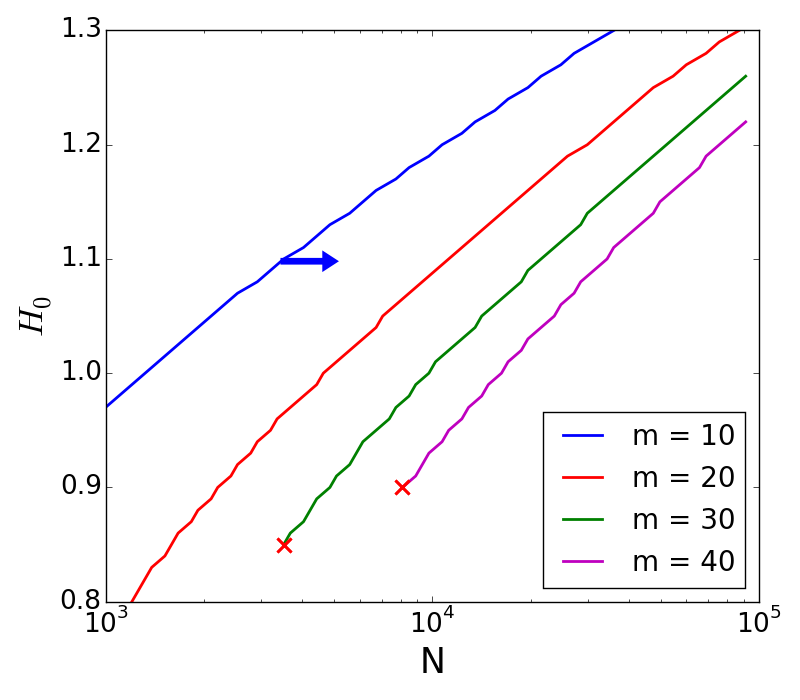
\includegraphics[width=\textwidth]{Figures/1_segregation_zone.png}
        \caption{Segregation domains}
        \label{Fig:1_segregation_zone}
    \end{subfigure}
\caption{(a): growth of perturbation $\xi_*$ over dimensionless time $\tau$ until the end of expansion at $\tau = 3.84$. An overdensity seeded with a wavelength $\lambda_*$ begins its collisional evolution when $\xi_*$ reaches $\frac{\lambda_*}{2}$. These regimes are illustrated for $\lambda_* =0.04$ and  $\lambda_* =0.08$. The overdensities have to evolve collisionally for at least $\tau_{ms}$ to mass-segregate. This time-scale is also shown for each case. The blue case evolve collisionally for several $\tau_{ms}$ and will end up mass-segregated, while the red case visibly don't have have time to segregate. Modes of large wavelength tend to produce less mass-segregated clumps. (b) for a given number of nodes $m$, a model on the right of the corresponding line (arrow for $m=10$) will have mass-segregated overdensities at the end of the expansion, will on the left, the collisional evolution is too short for segregation to sets in. The red crosses show the minimum N below which the modes cannot be resolved.} 
\label{Fig:0_perturbation_growth}
\end{figure}


We now make use of all previous development to follow the evolution of a perturbation in a given system and assess its dynamical state.

To ease comparisons with N-body calculations cast in standard H\'enon units, we set ${\cal M} = G = R_o = 1 $ and use $\Hub_0 = 1.0833 .. \simeq 1$ so that the total binding energy $E = -1/4$, which gives a value of $\Estar \simeq 6/7$. The Hubble expansion proceeds until a time $t = \tau / \Hub_0 \simeq 3.87 / \Hub_0$, when $H = 0$ and the bounding radius $R$ reaches $R = a(\tau)R_o \simeq 2.4 R_o$. The evolution time up to that point coincides almost exactly with the {\it current} global system free-fall time of $\approx 4.1$ time units. System-wide collapse to the barycentre will ensue on the same time-scale, but now this process will involve the merging / scattering of several high-density clumps. 

For simplicity, and for ease of calculations, we chose the mass of individual stars to follow a  truncated \cite{Salpeter1955} distribution function, where the distribution function $ dN/dm \propto m_\star^{-\alpha}$ with index $\alpha = 2.35$ for masses in the range  $0.3 M_\odot < m_\star < 100 M_\odot$ giving a mean value of $\simeq 1 M_\odot$.


We set $\Hub_0 = 1$ and $N = 15 000$ as reference\footnote{The more accurate value is $\Hub_0 = 1 + 1/12 = 1.0833$ but we rounded up to 1 to simplify the discussion}. We compute a mean initial amplitude of perturbation $\xistaro \approx 0.005 $ with a shortest-resolved wavelength $\lambda_\ast \approx 0.04$. Fig.~\ref{Fig:1_tau_ms} displays the solution from integrating Eqs.~(\ref{Eq:1_system}). The amplitude $\xistar(\tau)$ grows monotonically and crosses the values $\lambda_\ast/2$ at $\tau \approx 2.3$~: thereafter the perturbation enters a non-linear regime of evolution during which the internal dynamics may become collisional $( \Delta\tau > \tau_{ms})$. A second case is depicted on Fig.~\ref{Fig:1_tau_ms}, where the wavelength $\lambda_\ast = 0.08$ and the perturbation reaches amplitude $\xistar = \lambda_\ast/2$ at $\tau \approx 3.6$: there is then too little time left before the end of the Hubble expansion phase for a clump of stars to evolve collisionally ($\Delta\tau < \tau_{ms}$). 





The dynamical state of individual clumps is clearly a question of membership $N_\lambda$ and mass spectrum as shown in (\ref{Eqn:Taums}). We have been arguing that most small-size clumps will show collisional internal evolution~: a small cluster of stars would lose low-mass stars in the process and so have an increased ratio of average-    to maximum stellar mass. It is not clear, then, whether this trend is strong enough to compensate for the (almost) linear dependence on membership. 
%Anticipating the results of the next section, we take $N_\lambda$ from Eq.~(\ref{Eqn:Clumpn}) to compute  a product  $N_\lambda / \ln 0.4 N_\lambda \times \langle m_\ast\rangle / \max(m_\ast) \sim 14 $ for the case of a Salpeter mass function truncated at $20 M_\odot$ ;  and about $3$ for a truncation value of $100 M_\odot$. In practice, the results of N-body 
%calculations yielded values scattered in the range [3, 14] $M_\odot$, 
%consistent with there being {\it no trend}  with clump membership $N_\lambda$. To inspect further the actual properties of clumps, we next turn to  N-body calculations. 





\section{Concluding remarks}

We presented the recipe to build a \HubLem fragmented model. 

With an appropriate \tHub, below $\sqrt{2}$, the expansion of our model ends at a time we named apex time. We derived its expression as a function of \tHub, as well as the governing equations of the expansion. A perturbation analysis was performed to follow idealized radial overdensities. We expect clumps to undergo a phase of linear convergence followed by collisional evolution. We can also expect mass-segregation to occur in our clumps, though quantitative prediction cannot be obtained from idealized radial shell-like overdensities. N-body simulations are needed to obtain detailed characteristics.















